%======================================================================
\section{Track MOD --- Part modeling}\label{sec:mod}
%======================================================================

Modeling is the main track and comes first. M1 needs \eref{MOD-01}--\eref{MOD-05}, \eref{MOD-11} and
\eref{MOD-12}. Sheet metal and frames serve M3. Surfacing, freeform and mesh conversion are M5.

\begin{center}
\small
\begin{tabularx}{\linewidth}{@{}p{3.3cm}p{5.2cm}X@{}}
\toprule
Capability & FreeCAD 1.1.4 today (checked in this repo) & Gap to Fusion / SolidWorks\\
\midrule
Feature patterns & \code{LinearPattern} (2 directions), \code{PolarPattern}, \code{MultiTransform} & Bug in direction 2; no symmetric, no suppress\\
Body/component patterns & Draft link arrays & Not assembly-aware; no Fusion options\\
Parameters & Spreadsheet, \code{App::VarSet}, expressions & No Change Parameters dialog\\
Top-down & \code{ShapeBinder}, \code{SubShapeBinder} (cross-document) & No skeleton/derive workflow\\
Configurations & none (no configuration table in \file{src/Mod/Spreadsheet} or \file{src/App}) & Missing\\
Direct edit & \code{Part\_Defeaturing} (delete faces) & No press-pull, move or replace face\\
Threads & \code{Hole} has \code{ModelThread}; TechDraw draws cosmetic threads on views & No model-level cosmetic thread\\
Sheet metal & add-on only & Bundle (decided)\\
Weldments & none in core & Missing\\
Surfacing & Surface WB: Filling, Sections, GeomFillSurface, ExtendFace, BlendCurve; Part: Ruled, Offset, Thickness & Trim/untrim, stitch, continuity analysis\\
Freeform & none & Missing\\
Mesh $\rightarrow$ solid & \code{Part\_ShapeFromMesh} (faceted), ReverseEngineering WB & No segmentation/rebuild\\
Inspect & Measure incl.\ \code{MeasureCOM}; \code{Part\_CheckGeometry} & No overhang/draft/thickness maps\\
\bottomrule
\end{tabularx}
\end{center}

%----------------------------------------------------------------------
\subsection{BW-MOD-01 --- Rectangular and circular patterns}\label{sec:patterns}
%----------------------------------------------------------------------

\begin{epic}{MOD-01}{Rectangular \& circular patterns}{M1}{\stProg}{(new, from the UI plan)}
Two commands under \textsc{Create}: Rectangular Pattern and Circular Pattern. Each works on features,
bodies and assembly components, with Fusion's options: symmetric direction, suppress instances, and linked
vs.\ independent copies (linked by default). Depends on \eref{FND-06} (the direction-2 fix).
\emph{Acceptance:} Figures~\ref{fig:examples} and \ref{fig:new} reproduced in the GUI; undo/redo;
save/reload; the Assembly workbench sees every component instance.
\end{epic}

\begin{center}
\small
\begin{tabularx}{\linewidth}{@{}p{3.4cm}XX@{}}
\toprule
Fusion option & FreeCAD 1.1 today & Plan\\
\midrule
Pattern type: Features & PartDesign \code{LinearPattern} (2 directions), \code{PolarPattern} & Wrap these, fix the direction-2 bug\\
Pattern type: Bodies & Draft \code{make\_ortho\_array} / \code{make\_polar\_array} with \code{use\_link} & New command builds a link array, or copies\\
Pattern type: Components & Assembly understands link arrays (\file{UtilsAssembly.py:127--131}) & New command builds an \code{App::Link} array inside the assembly\\
Distance type: Extent / Spacing & \code{Mode} = Extent / Spacing & Same\\
Direction type: Symmetric & --- & \textbf{New}: index range $-\lfloor\frac{n-1}{2}\rfloor..\lceil\frac{n-1}{2}\rceil$\\
Circular type: Full / Angle / Symmetric & Angle + Extent/Spacing & Map Full/Angle; \textbf{new} Symmetric\\
Suppress instances & --- (features) & \textbf{New} for features; links: \code{setElementVisible}\\
Linked / independent & n/a & Dialog option (bodies, components)\\
\bottomrule
\end{tabularx}
\end{center}

\begin{figure}[ht]
\centering
\begin{subfigure}{0.49\linewidth}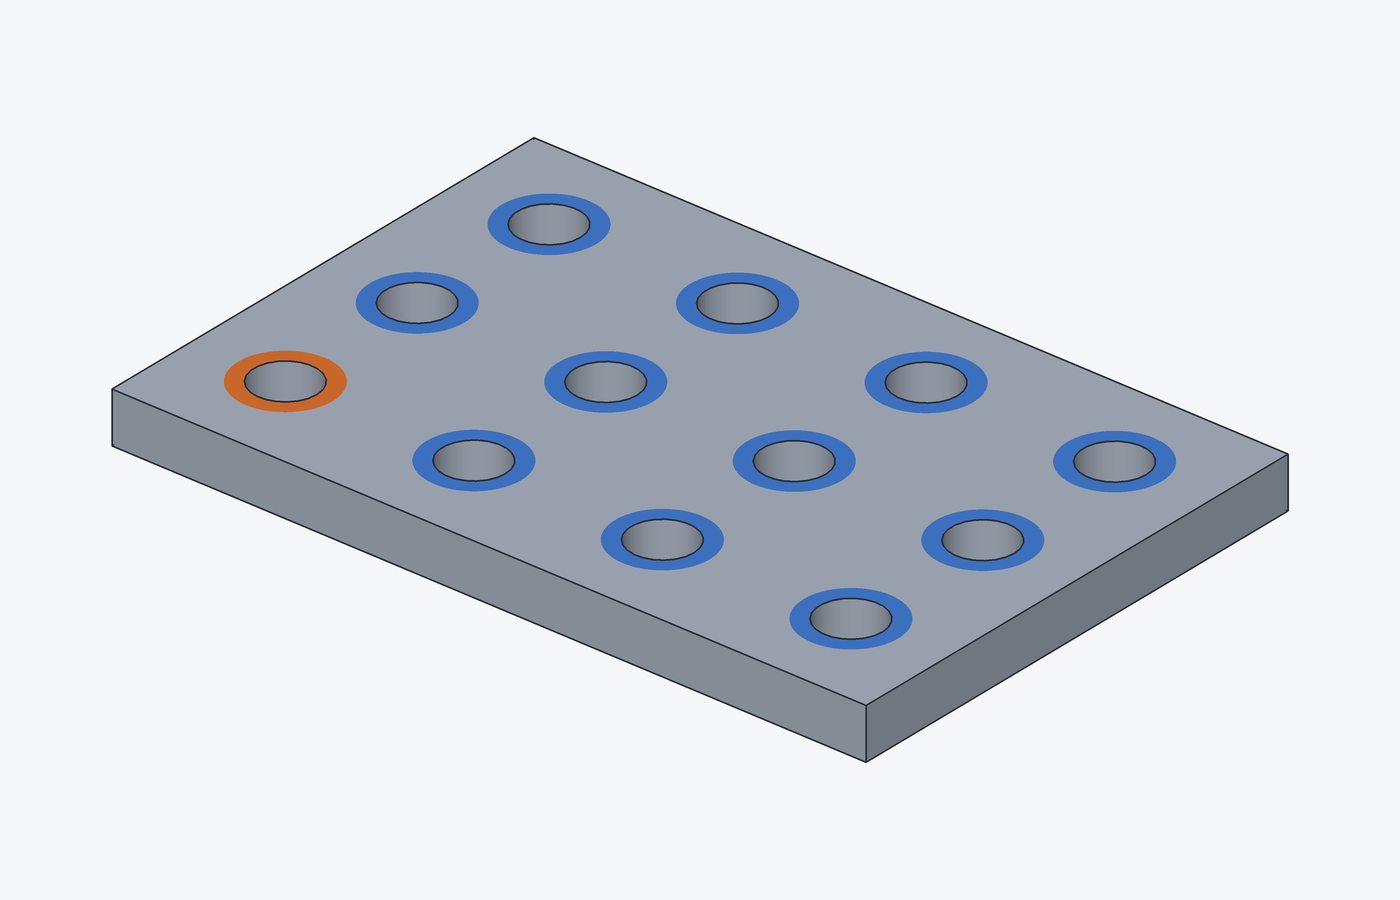
\includegraphics[width=\linewidth]{fig/rect_feature.png}
  \caption{Feature, rectangular: $4\times3$ holes (\code{LinearPattern}, two directions).}\end{subfigure}\hfill
\begin{subfigure}{0.49\linewidth}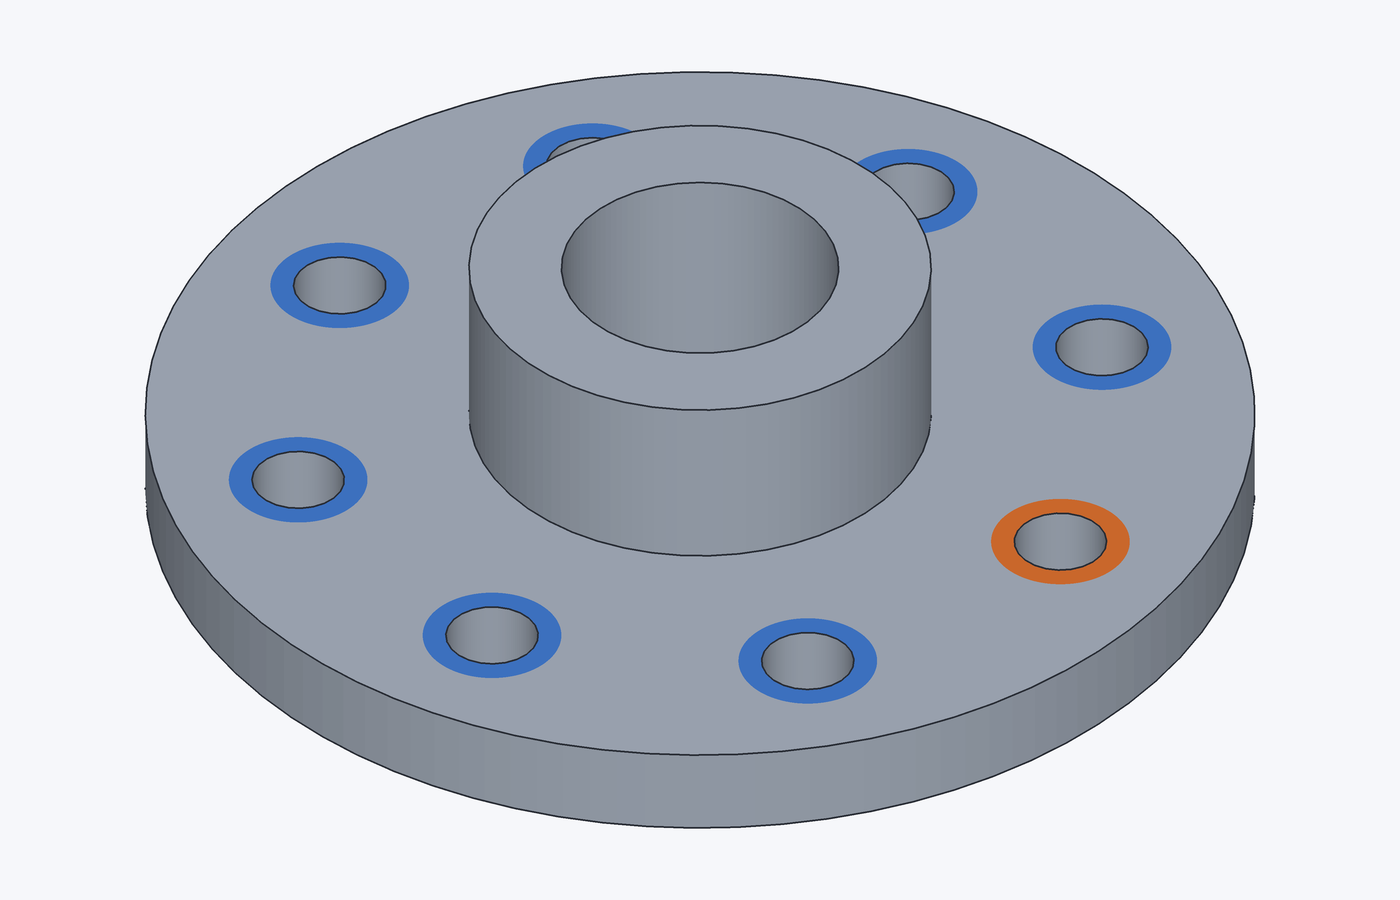
\includegraphics[width=\linewidth]{fig/circ_feature.png}
  \caption{Feature, circular: 8 bolt holes (\code{PolarPattern}, Full).}\end{subfigure}\\[4pt]
\begin{subfigure}{0.49\linewidth}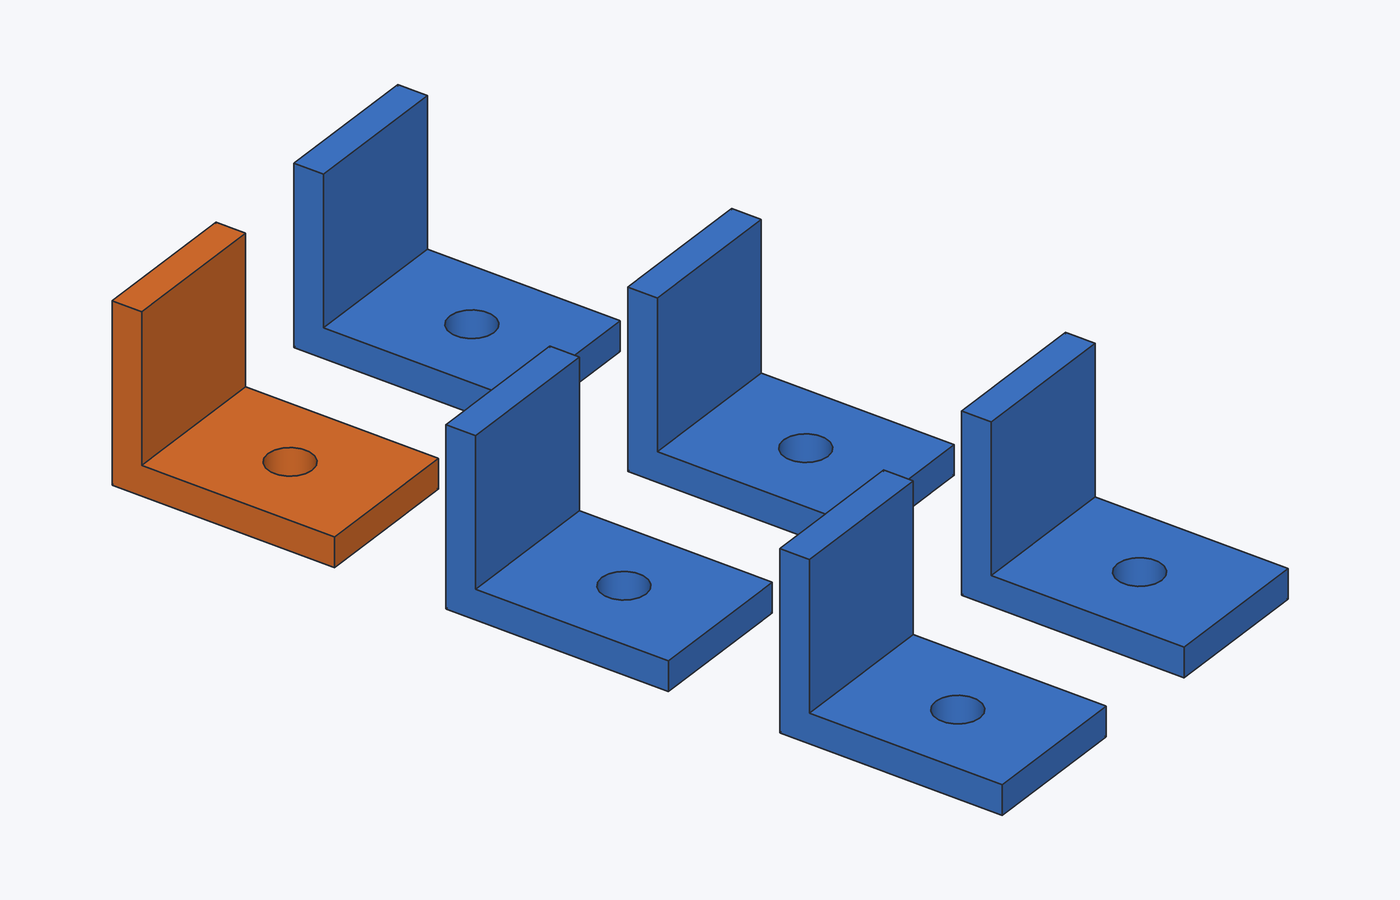
\includegraphics[width=\linewidth]{fig/body_pattern.png}
  \caption{Bodies, rectangular: $3\times2$ brackets (link array).}\end{subfigure}\hfill
\begin{subfigure}{0.49\linewidth}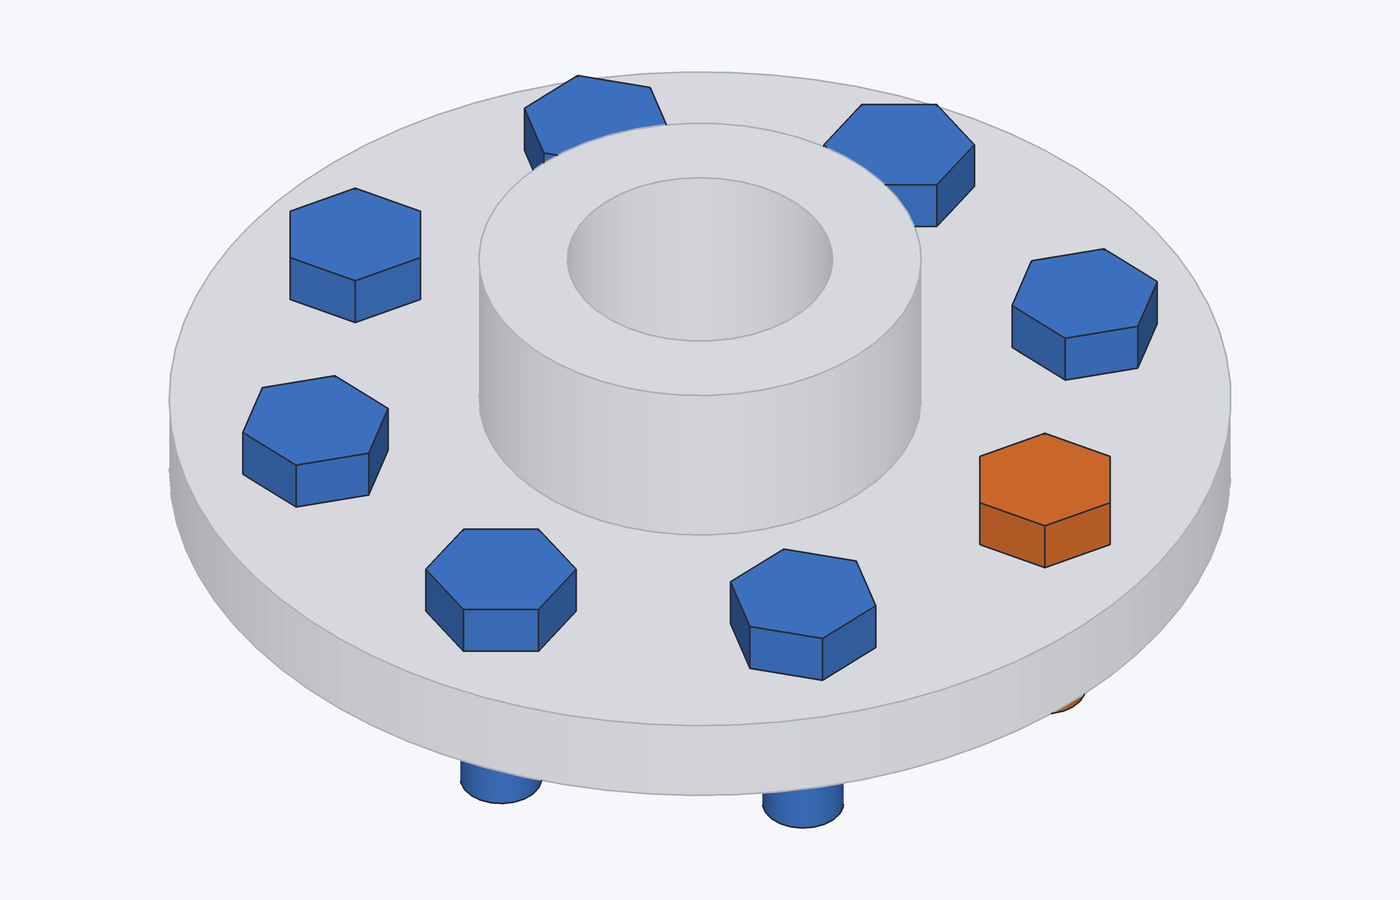
\includegraphics[width=\linewidth]{fig/component_pattern.png}
  \caption{Components, circular: 8 bolts around the flange axis.}\end{subfigure}
\caption{Pattern examples. Seed in \textcolor{bworange}{orange}, generated instances in
\textcolor{bwblue}{blue}. Panels (a) and (b) are real PartDesign features recomputed in headless FreeCAD
1.1.4 (panel (a) with the direction-2 workaround). Panel (c) was built with Draft's link array (6 elements
confirmed). Panel (d) uses the same transforms as the component command.}
\label{fig:examples}
\end{figure}

\subsubsection*{Theory}

\paragraph{Rigid motions.} An instance is the seed moved by a rigid motion $g\in SE(3)$,
\[
  g = \begin{pmatrix} R & \mathbf t\\ \mathbf 0^{\!\top} & 1\end{pmatrix},\qquad
  R\in SO(3),\ \mathbf t\in\mathbb R^3 .
\]
A pattern is a finite family $\{g_k\}_{k\in K}$ with $g_{\mathbf 0}=I$ (the seed). Features change one solid
with Booleans, $S\cup\bigcup_{k\neq 0} g_k(T)$ (additive) or $S\setminus\bigcup_{k\neq0} g_k(T)$
(subtractive), where $S$ is the support and $T$ the seed's tool shape. Bodies and components only produce
\emph{placements} $\{g_k P_0\}$, so no Boolean is evaluated.

\paragraph{Rectangular lattice.} With unit directions $\mathbf u_1,\mathbf u_2$ and per-gap spacings
$s^{(a)}_q$,
\[
  \mathbf t_{ij} = d_1(i)\,\mathbf u_1 + d_2(j)\,\mathbf u_2,\qquad
  d_a(m) = \operatorname{sgn}(m)\sum_{q=1}^{|m|} s^{(a)}_q .
\]
In \emph{Extent} mode $s_a = L_a/(n_a-1)$, and in \emph{Spacing} mode $L_a=(n_a-1)s_a$. These are
\code{calculateOffsetVector} and \code{calculateSteps} in \file{FeatureLinearPattern.cpp}. The index sets are
$I_a^{\text{one}}=\{0,\dots,n_a-1\}$ and $I_a^{\text{sym}}=\{-\lfloor\tfrac{n_a-1}{2}\rfloor,\dots,\lceil\tfrac{n_a-1}{2}\rceil\}$,
and $K=(I_1\times I_2)\setminus K_{\text{supp}}$. Translations commute, so the order of the two directions is
irrelevant. Instances are distinct iff every $s^{(a)}_q\neq0$ and $\mathbf u_1\nparallel\mathbf u_2$. The
bug below breaks the first condition.

\paragraph{Circular pattern.} About an axis through $\mathbf c$ with direction $\mathbf a$, Rodrigues'
formula gives
$R(\mathbf a,\theta) = I + \sin\theta\,[\mathbf a]_\times + (1-\cos\theta)\,[\mathbf a]_\times^2$ and
$g_k:\mathbf p\mapsto\mathbf c+R(\mathbf a,\theta_k)(\mathbf p-\mathbf c)$. The schedule is
$\theta_k = 2\pi k/n$ for \emph{Full} (dividing by $n$, since $2\pi\equiv0$), and
$\theta_k=\Theta k/(n-1)$ for \emph{Angle} ($k\in I^{\text{one}}$) and \emph{Symmetric}
($k\in I^{\text{sym}}$). Rotations about different axes do not commute, so nested patterns use a fixed
order, $g=g^{\text{outer}}_k\,g^{\text{inner}}_{ij}$.

\paragraph{Placements.} Pattern transforms are defined in world coordinates, so instance placements are
the left product $P_k=g_kP_0$. The right product $P_0g_k$ would pattern in the seed's local frame.

\paragraph{Linked vs.\ independent.} A link array stores the seed B-rep once plus $n$ placements,
$O(|B|+n)$ memory, and follows edits. Independent copies cost $O(n|B|)$. Verified headless:
\code{App::Link} with \code{ElementCount}$=8$ produced 8 \code{App::LinkElement}s and a compound of 8
solids. \code{setElementVisible("3", False)} dropped it to 7, which gives suppression for bodies and
components with no new code.

\paragraph{Compute modes.} Fusion's \emph{Identical} equals FreeCAD's \code{TransformMode = Features}
(the tool shape is copied). \emph{Adjust} re-evaluates each instance's terminations and needs a re-execute per
instance, so it is deferred (\S\ref{sec:questions}).

\begin{figure}[ht]
\centering
\begin{subfigure}{0.49\linewidth}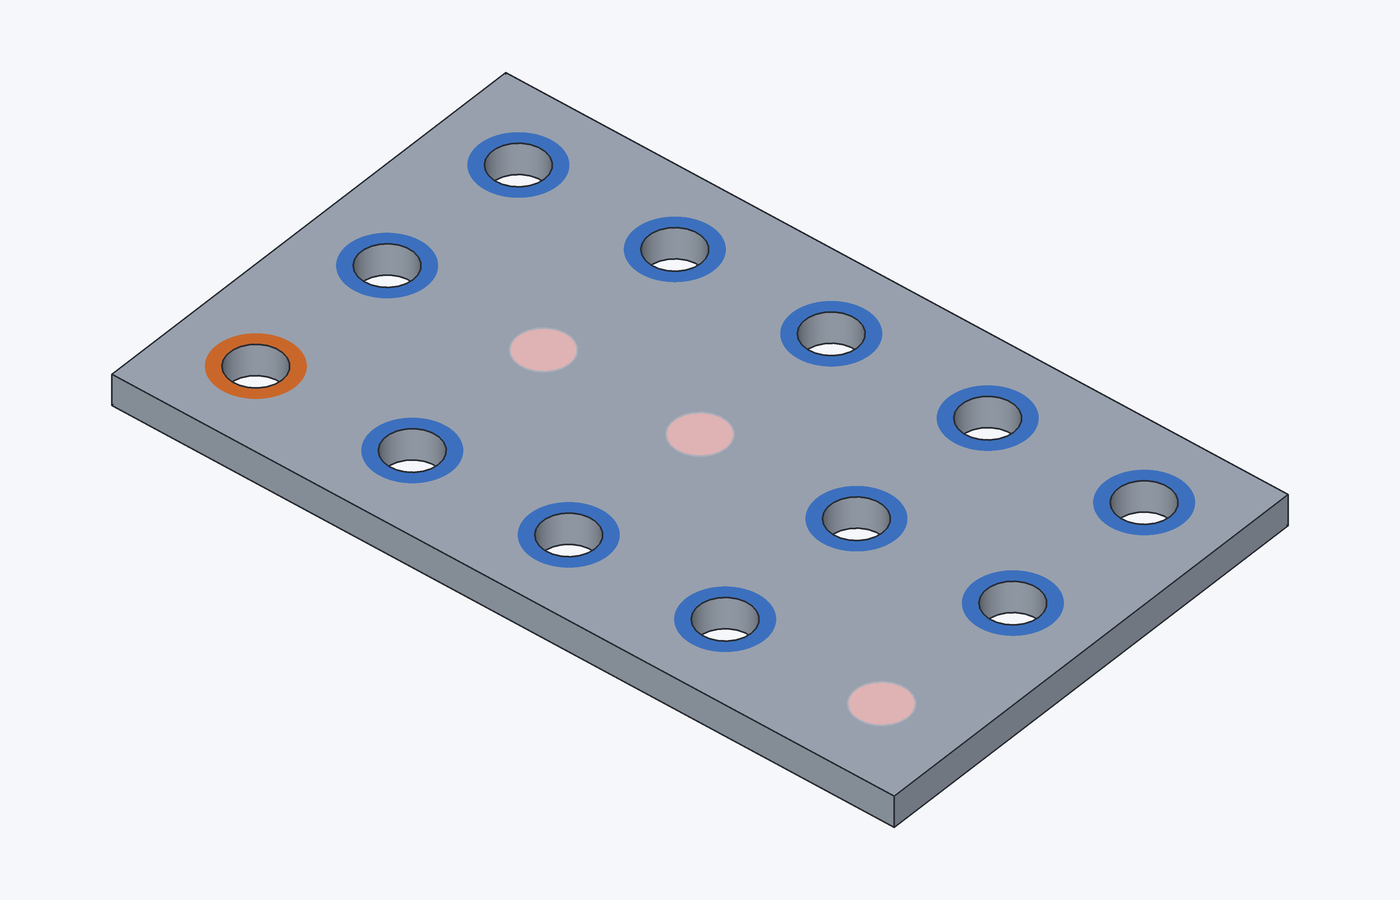
\includegraphics[width=\linewidth]{fig/suppression.png}
  \caption{Suppression: $K=(I_1\times I_2)\setminus K_{\text{supp}}$, $|K|=12$.}\end{subfigure}\hfill
\begin{subfigure}{0.49\linewidth}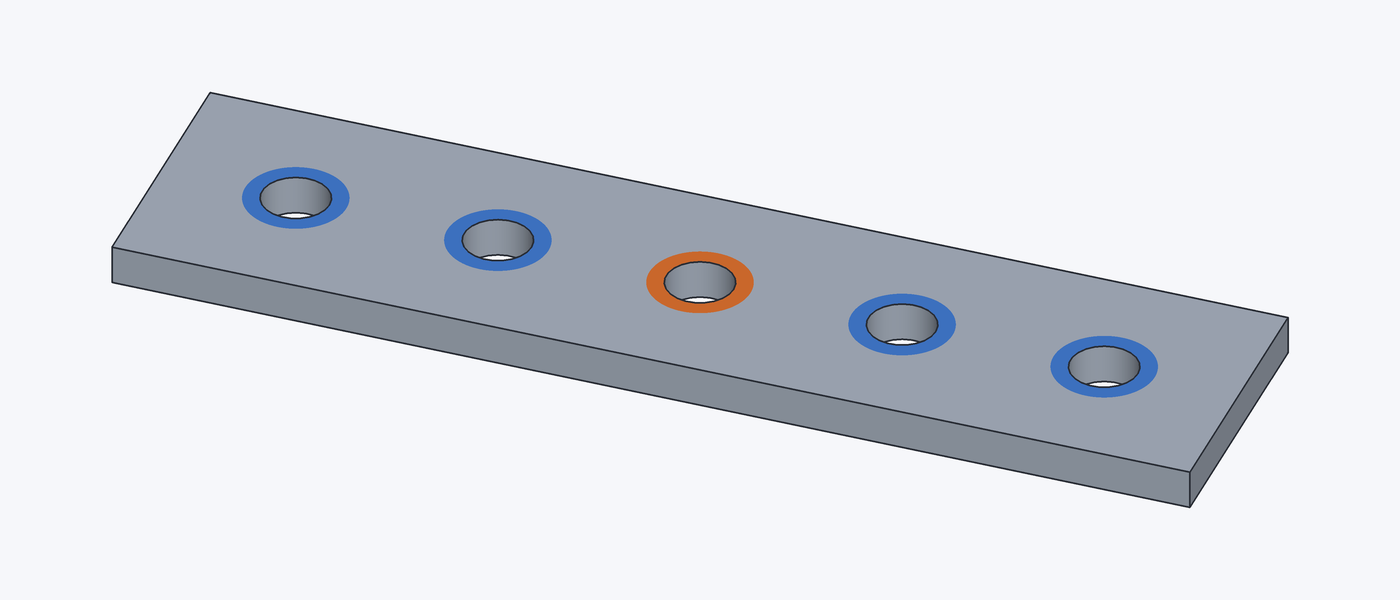
\includegraphics[width=\linewidth]{fig/symmetric.png}
  \caption{Symmetric direction, $n=5$: $I=\{-2,\dots,2\}$.}\end{subfigure}
\caption{The two new pattern options (target behaviour, not output of existing FreeCAD features).}
\label{fig:new}
\end{figure}

\paragraph{The direction-2 bug.}\label{sec:bug}
\begin{center}
\small
\begin{tabular}{@{}lccc@{}}
\toprule
Probe (headless FreeCAD 1.1.4) & rows asked & rows made & \code{Spacings2}\\
\midrule
Spacing 25\,mm, $n_2=3$ & 3 & 2 ($y=15,40$) & \code{[0.0, -1.0]}\\
Extent 50\,mm, $n_2=3$ & 3 & 3 & \code{[0.0, -1.0]}\\
Spacing 25\,mm, $n_2=5$ & 5 & 4 & \code{[0.0, -1.0, -1.0, -1.0]}\\
Direction 1, Spacing 30\,mm, $n_1=4$ & 4 & 4 & (\code{Spacings} correct)\\
\bottomrule
\end{tabular}
\end{center}
\begin{lstlisting}[language=C++]
ADD_PROPERTY_TYPE(Spacings,  ({-1.0}), "Direction 1", ...);  // ok
ADD_PROPERTY_TYPE(Spacings2, ({}),     "Direction 2", ...);  // {} -> setValue(double{}) -> [0.0]
\end{lstlisting}
The leading $0.0$ survives \code{updateSpacings}, so the first cumulative step is zero and a duplicate row
lands on the seed. Fixed on 19 Oct 2026: declared \code{(\{-1.0\})}, normalised in the constructor (as upstream main now
does), and a stored $0$ is mapped to $-1$ and written back, which repairs saved files. Three regression tests
(spacing, extent, old-file repair); all 171 PartDesign tests pass. Upstream main still declares
\code{(\{\})}; its constructor masks the bug for new objects but not for saved files, so the repair is worth
upstreaming (\eref{FND-06}).

\paragraph{Commands (built 19 Oct 2026, in GUI testing).} \code{BruceWorx\_RectangularPattern} and
\code{BruceWorx\_CircularPattern} (\file{bruceworx\_pattern.py}, \file{bruceworx\_pattern\_gui.py}) dispatch on
the selection. \emph{PartDesign features} go to PartDesign's own Linear/Polar Pattern. \emph{Bodies, Part
solids and assembly components} get an \code{App::Link} array whose parameters are dynamic properties in a
``BruceWorx Pattern'' group: rectangular (two directions, spacing or extent, symmetric) or circular (full,
angle, symmetric; axis from X/Y/Z, a straight edge, a circular edge's centre or a datum axis), suppression
per instance, and linked or independent copies. A task panel previews live, and Cancel removes everything
with or without document undo. Moving the seed re-places the pattern. In an assembly, the array's elements
count as components (\code{UtilsAssembly.isLinkGroup}; verified 6 components for a 6-up bolt pattern).
19 headless tests plus offscreen dialog smoke tests.

\paragraph{Upstream changes the feature path.} Upstream \code{main} (June--October 2026, PRs \#30417 and
\#32843) moved Linear/Polar Pattern logic into \code{Part::LinearPatternExtension} and friends and added
per-instance suppression (\code{SuppressedPositions}). Symmetric directions and suppression for
\emph{features} are therefore taken from upstream after the rebase (\eref{FND-03}), not written again on
1.1.4. Symmetric for features remains a candidate upstream contribution.

\begin{figure}[ht]
\centering
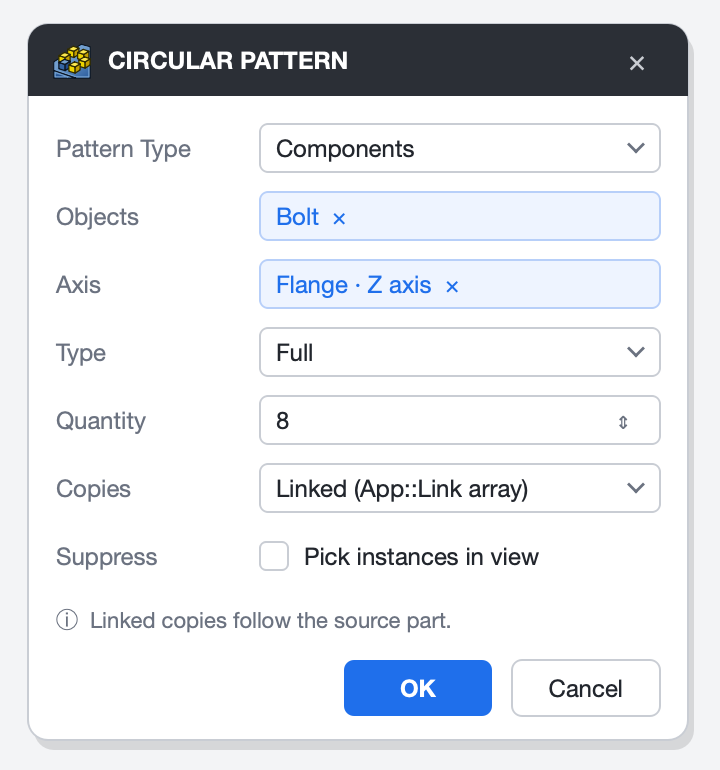
\includegraphics[width=0.36\linewidth]{fig/dialog_circ.png}
\caption{Circular Pattern dialog for components (working mock). \emph{Copies} shows for bodies and
components; \emph{Compute} only for features.}
\end{figure}

%----------------------------------------------------------------------
\subsection{BW-MOD-02 --- Parameters and top-down design}
%----------------------------------------------------------------------

\begin{epic}{MOD-02}{Parameters \& top-down design}{M1}{\stTodo}{(new)}
\begin{itemize}
  \item \textbf{Change Parameters} dialog (Fusion's name) listing every user parameter with its expression,
        value, unit and comment, drawn from \code{VarSet}s, Spreadsheet aliases and named feature
        dimensions, with search and favourites.
  \item \textbf{Skeleton} workflow: a master sketch or skeleton part drives layout, and parts consume it
        through \code{SubShapeBinder} across files. That fits the one-file-per-part model (\eref{ASM-01}).
  \item \textbf{Derive}: bring selected bodies, sketches or parameters from another file in as a linked,
        read-only reference, like SolidWorks' Insert Part or Fusion's Derive.
\end{itemize}
\emph{Acceptance:} changing a skeleton dimension updates three linked part files in one recompute.
\end{epic}

\paragraph{Theory: the recompute graph.} A document is a directed graph $G=(V,E)$ with an edge $u\to v$
when $v$ reads $u$ through a link or an expression. Recompute evaluates $V$ in a topological order of $G$,
in $O(|V|+|E|)$ time, and only for the \emph{touched} set's descendants. Top-down design adds edges
\emph{between documents}. The combined graph must stay acyclic. A part that binds geometry from an assembly
which contains that same part would close a cycle $p\to a\to p$. The tooling therefore refuses that
binding up front, rather than letting recompute fail. It allows a skeleton part referenced by both instead.

%----------------------------------------------------------------------
\subsection{BW-MOD-03 --- Configurations}
%----------------------------------------------------------------------

\begin{epic}{MOD-03}{Configurations}{M1}{\stTodo}{(new)}
One part or assembly file holds several variants (Fusion: Configurations; SolidWorks: configurations and
design tables). A \textbf{configuration table} object has rows for configurations and columns for parameters,
feature suppression states, custom properties (including the part number), and for assemblies, which
configuration each component uses. Activating a row writes the values and recomputes.
\emph{Acceptance:} Short, Standard and Long brackets come from one file
(Figure~\ref{fig:cfg}), and the BOM lists each configuration's own P/N.
\end{epic}

\begin{figure}[ht]
\centering
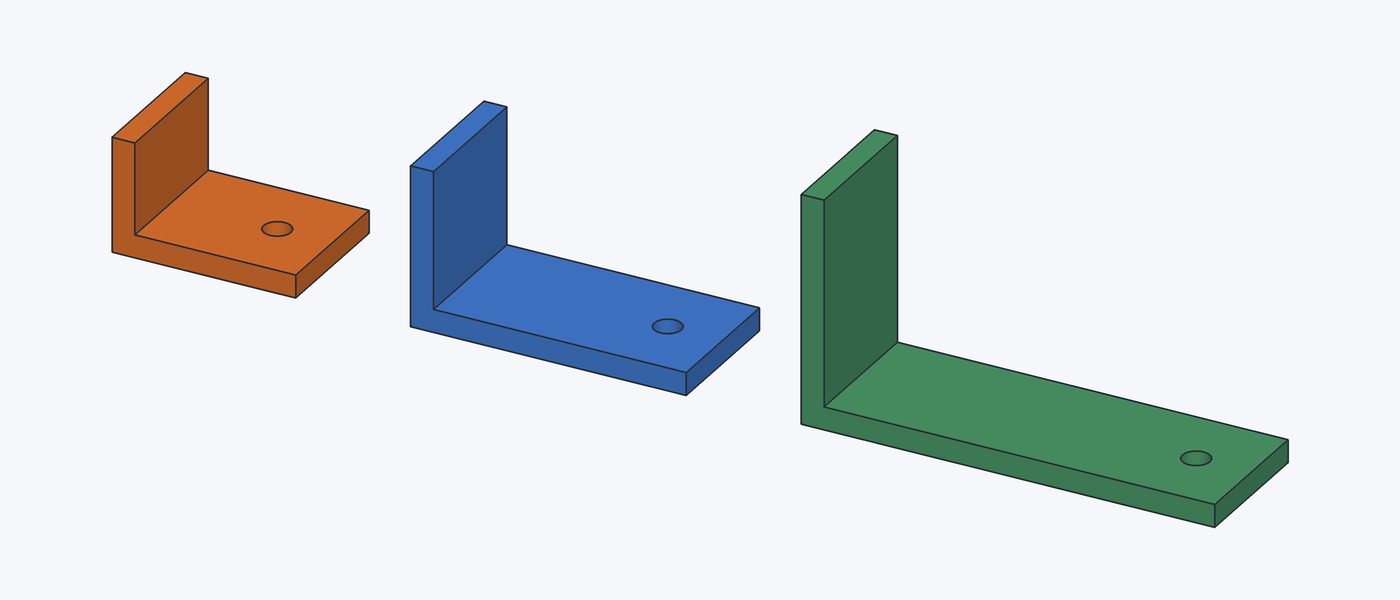
\includegraphics[width=0.85\linewidth]{fig/cfg_bracket.png}
\caption{Three configurations of one PartDesign body. A \code{VarSet} drives \code{Length}, \code{Height}
and the hole position by expression, and recomputing with three value sets gives volumes of
8\,858.6, 13\,358.6 and 20\,108.6\,mm$^3$. This is the mechanism the configuration table automates.
Built by \file{scripts/render\_roadmap.py}.}
\label{fig:cfg}
\end{figure}

\paragraph{Theory.} Let $\mathbf p\in\mathcal P$ be the parameter vector and $\mathbf s\in\{0,1\}^{F}$
the suppression state of $F$ features. A configuration is $c_j=(\mathbf p_j,\mathbf s_j,\pi_j)$, where
$\pi_j$ holds its properties (P/N, description, material). The model is a function $M(\mathbf p,\mathbf s)$
evaluated by recompute. Configurations change \emph{inputs only}, never topology of the feature graph, so
one history serves all rows. Two consequences follow:
\begin{enumerate}
  \item Each configuration is a distinct item for manufacturing, so it carries its \textbf{own P/N}. The BOM
        resolves a component to $(\text{file},c_j)$, not just to a file.
  \item Topological naming must survive a row switch. A fillet on an edge that exists only when a feature is
        unsuppressed has to be suppressed in the rows where that edge is missing. Per-row validation runs
        every configuration in CI and reports which features fail in which rows.
\end{enumerate}
Storage: a \code{BruceWorx::ConfigurationTable} object (FeaturePython) in the part file. It can import and
export CSV, so variants can be edited in a spreadsheet, as with a SolidWorks design table.

%----------------------------------------------------------------------
\subsection{BW-MOD-04 --- Direct edit on imported geometry}
%----------------------------------------------------------------------

\begin{epic}{MOD-04}{Direct edit on imported geometry}{M1}{\stTodo}{FCB-P2-15}
Edit ``dumb'' solids from STEP (Fusion exports, vendor parts) without a feature history:
\textbf{delete face} (exists: \code{Part\_Defeaturing}), \textbf{press-pull / offset face},
\textbf{move face} (translate or rotate), \textbf{replace face} (with a surface), plus \textbf{feature
recognition} that turns cylindrical cut faces into editable holes. Each edit is a parametric feature on top
of the imported shape, so it appears in the timeline.
\emph{Acceptance:} the Fusion STEP of \code{LE-01001} has a hole moved and a face offset, and stays valid.
\end{epic}

\begin{figure}[ht]
\centering
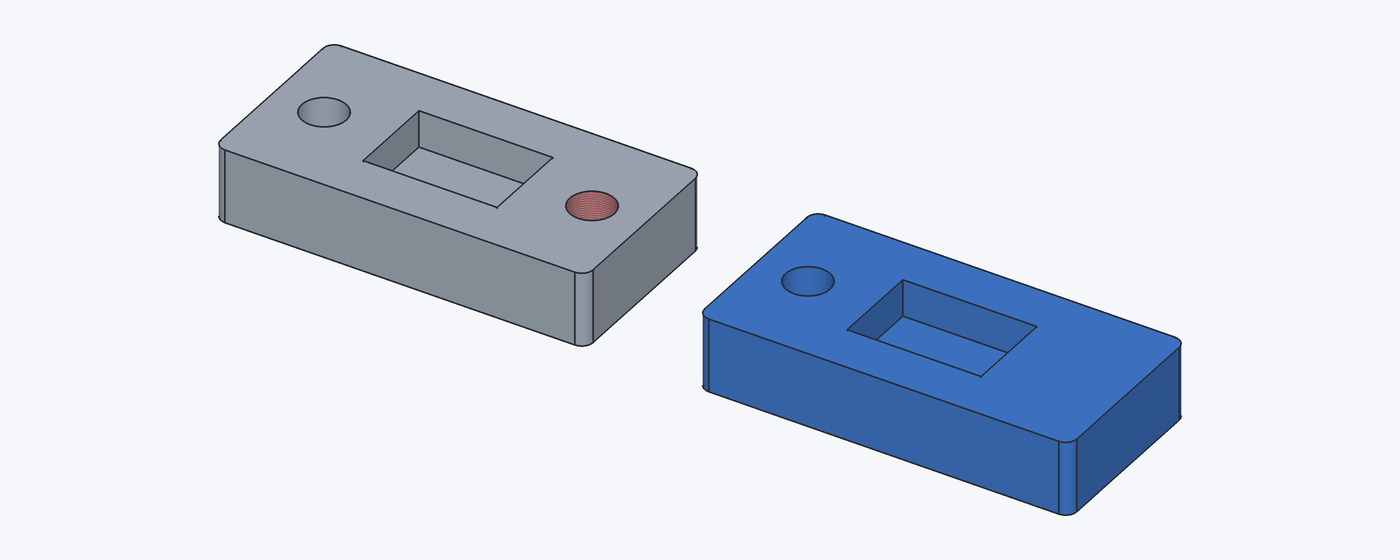
\includegraphics[width=0.85\linewidth]{fig/direct_edit.png}
\caption{Direct edit available today. A filleted block is exported to STEP and re-imported as a dumb solid
(17 faces). The right-hand hole's faces (red) are removed with \code{Shape.defeaturing} in headless
FreeCAD, giving 16 faces and a valid solid (blue). Press-pull, move and replace face build on the same kind of
local operation.}
\label{fig:direct}
\end{figure}

\paragraph{Theory: local face offset.} Press-pull replaces a face $F$ on surface $S(u,v)$ with its offset
$S_d(u,v)=S(u,v)+d\,\mathbf n(u,v)$, then re-intersects $S_d$ with the surfaces of the faces adjacent to $F$
to rebuild the edges, and extends or trims those neighbours. That is OCCT's
\code{BRepOffsetAPI\_MakeOffsetShape} in local mode, or \code{BRepFeat} for planar faces. Validity
conditions:
\begin{itemize}
  \item $|d|$ must stay below the minimum radius of curvature of $S$ where $d$ points to the concave side,
        or the offset self-intersects;
  \item each neighbour must still intersect $S_d$. A neighbour that ``runs out'' (a blend narrower than $d$)
        is removed first, which is how Fusion handles fillets that disappear when a face is pushed.
\end{itemize}
\textbf{Feature recognition:} cylindrical faces sharing an axis, with a closed boundary on a planar face,
become a hole candidate $(\mathbf c,\mathbf a,r,\text{depth})$. Counterbores are coaxial pairs with
$r_2>r_1$. The recognised hole is replaced by a real \code{Hole} feature, which also feeds drawing callouts
(\eref{DRW-04}).

%----------------------------------------------------------------------
\subsection{BW-MOD-05 --- Threads, holes and hardware}
%----------------------------------------------------------------------

\begin{epic}{MOD-05}{Threads, holes \& hardware library}{M1}{\stTodo}{FCB-P2-09/10, (new)}
\begin{itemize}
  \item \textbf{Cosmetic thread} object attached to a cylindrical face, storing standard, size, pitch,
        class, length, and handedness. It is shown in 3D as a texture/helix decoration, exported in STEP
        AP242 PMI where supported, and read by TechDraw for callouts.
  \item \textbf{Hole presets} (Hole Wizard parity): clearance (close/normal/loose), tapped, counterbore
        and countersink per fastener, plus \textbf{heat-set insert} holes by insert part number, the common
        case for FDM parts.
  \item \textbf{Fastener library}: evaluate the FreeCAD Fasteners add-on (licence and maintenance
        \verify) against a BruceWorx library built on the COTS schema (\eref{ROB-01}).
\end{itemize}
\emph{Acceptance:} an M3 tapped hole and an M3 heat-set hole both produce correct callouts on the drawing.
\end{epic}

\paragraph{Theory: thread geometry.} For ISO metric threads of nominal diameter $d$ and pitch $P$, the
fundamental triangle height is $H=\tfrac{\sqrt3}{2}P$. The basic internal minor diameter is
$D_1=d-2\cdot\tfrac{5}{8}H = d-1.0825\,P$, and the external minor diameter is $d_3=d-1.2269\,P$. Tap drill
$\approx d-P$ (M3$\times$0.5 $\rightarrow$ 2.5\,mm). A cosmetic thread stores $(d,P,\text{class},L)$ and draws
the minor/major diameter circle in views. Modelled threads (\code{ModelThread}) are kept for 3D printing,
where the printed geometry is the thread.

%----------------------------------------------------------------------
\subsection{BW-MOD-06 --- Sheet metal}
%----------------------------------------------------------------------

\begin{epic}{MOD-06}{Sheet metal}{M3}{\stTodo}{(new, from the UI plan)}
Bundle the SheetMetal add-on (decided; LGPL-2.1-or-later since v0.4.00) and add per-material, per-thickness
\textbf{rules} (bend radius, K-factor, relief) as a library, like Fusion's sheet-metal rules. Flats and
DXF are covered in \eref{MFG-03}, and the drawing in \eref{DRW-07}.
\emph{Acceptance:} the bracket in Figure~\ref{fig:sheet} unfolds to the length given by the bend-allowance
formula within 0.01\,mm.
\end{epic}

\begin{figure}[ht]
\centering
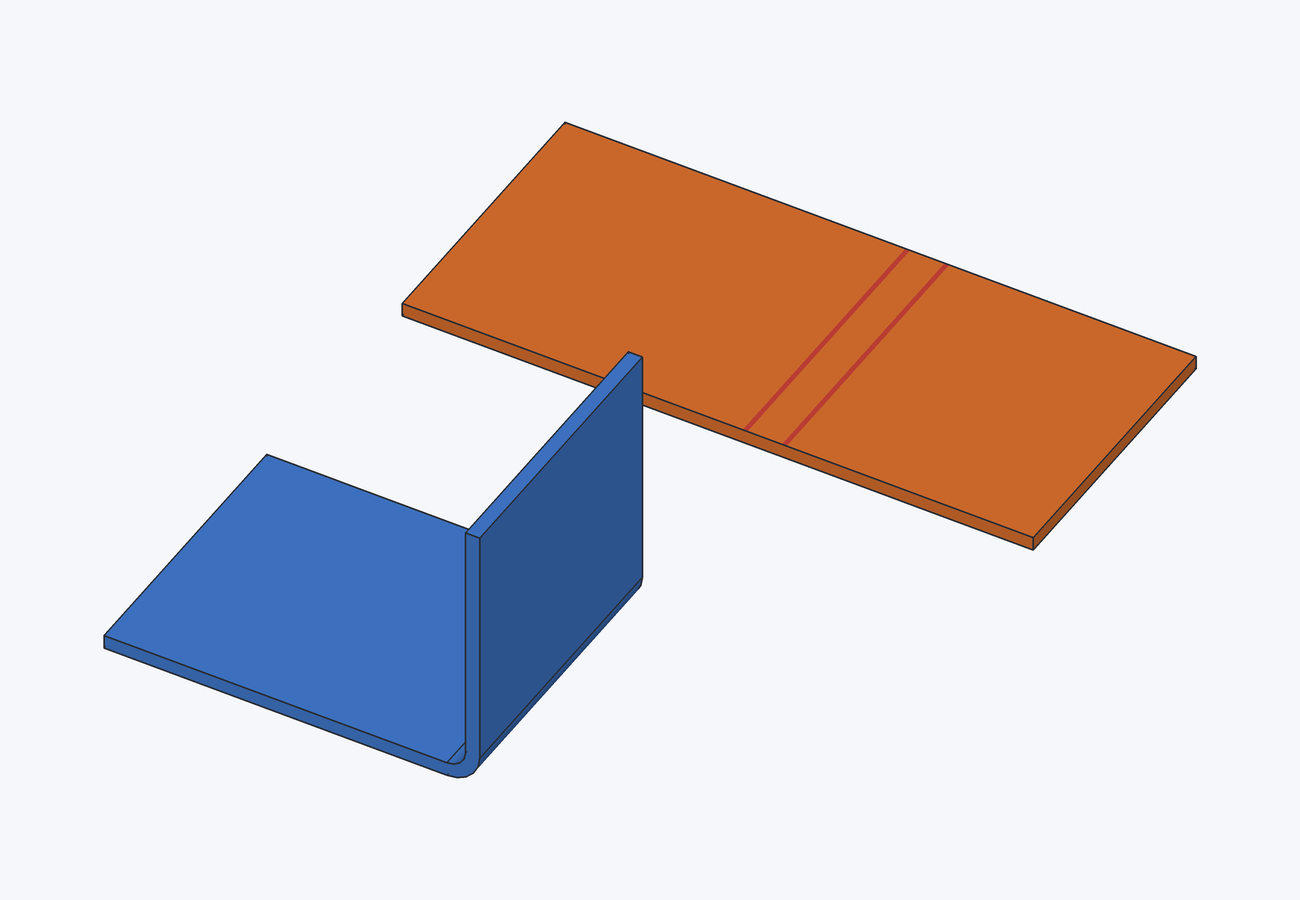
\includegraphics[width=0.62\linewidth]{fig/sheet_flat.png}
\caption{90$^\circ$ bracket (blue): $T=1.5$, $R_i=2$, outside flanges 40 and 30\,mm, depth 30\,mm, built as one
valid solid (volume 3\,029.4\,mm$^3$, matching the analytic value). Its flat (orange) is 67.178\,mm long, with
the bend zone between the red lines ($BA=4.178$\,mm at $K=0.44$).}
\label{fig:sheet}
\end{figure}

\paragraph{Theory: bend allowance.} During bending the neutral fibre sits at $R_i+KT$ from the bend axis,
with $0<K<0.5$ depending on material and process. Its arc length is the bend allowance
\[
  BA=\theta\,(R_i+K\,T),\qquad
  L_{\text{flat}} = \sum_i \ell_i + \sum_j BA_j ,
\]
where $\ell_i$ are the straight lengths between bend tangent lines. For the bracket,
$\ell_1=40-(2+1.5)=36.5$, $\ell_2=30-3.5=26.5$, and $BA=\tfrac{\pi}{2}(2+0.44\cdot1.5)=4.178$, so
$L_{\text{flat}}=67.178$\,mm. $K$ comes from the rules library per material, thickness and tooling. That is
why the rules table matters more than the unfold algorithm.

%----------------------------------------------------------------------
\subsection{BW-MOD-07 --- Frames and weldments}
%----------------------------------------------------------------------

\begin{epic}{MOD-07}{Frames \& weldments}{M3}{\stTodo}{(new)}
Structural members swept along 3D-sketch edges from a \textbf{profile library}: 2020/2040 aluminium
extrusion, square and round tube, angle, flat bar. Each joint gets an \textbf{end treatment} (mitre, butt
one or the other, cope), and \textbf{trim/extend} works against other members. The \textbf{cut list} groups
identical members and gives stock length, angles and quantity. Each member is a body with a cut-list item, not
a separate part file.
\emph{Acceptance:} the frame in Figure~\ref{fig:frame} produces the cut list below.
\end{epic}

\begin{figure}[ht]
\centering
\begin{minipage}{0.48\linewidth}
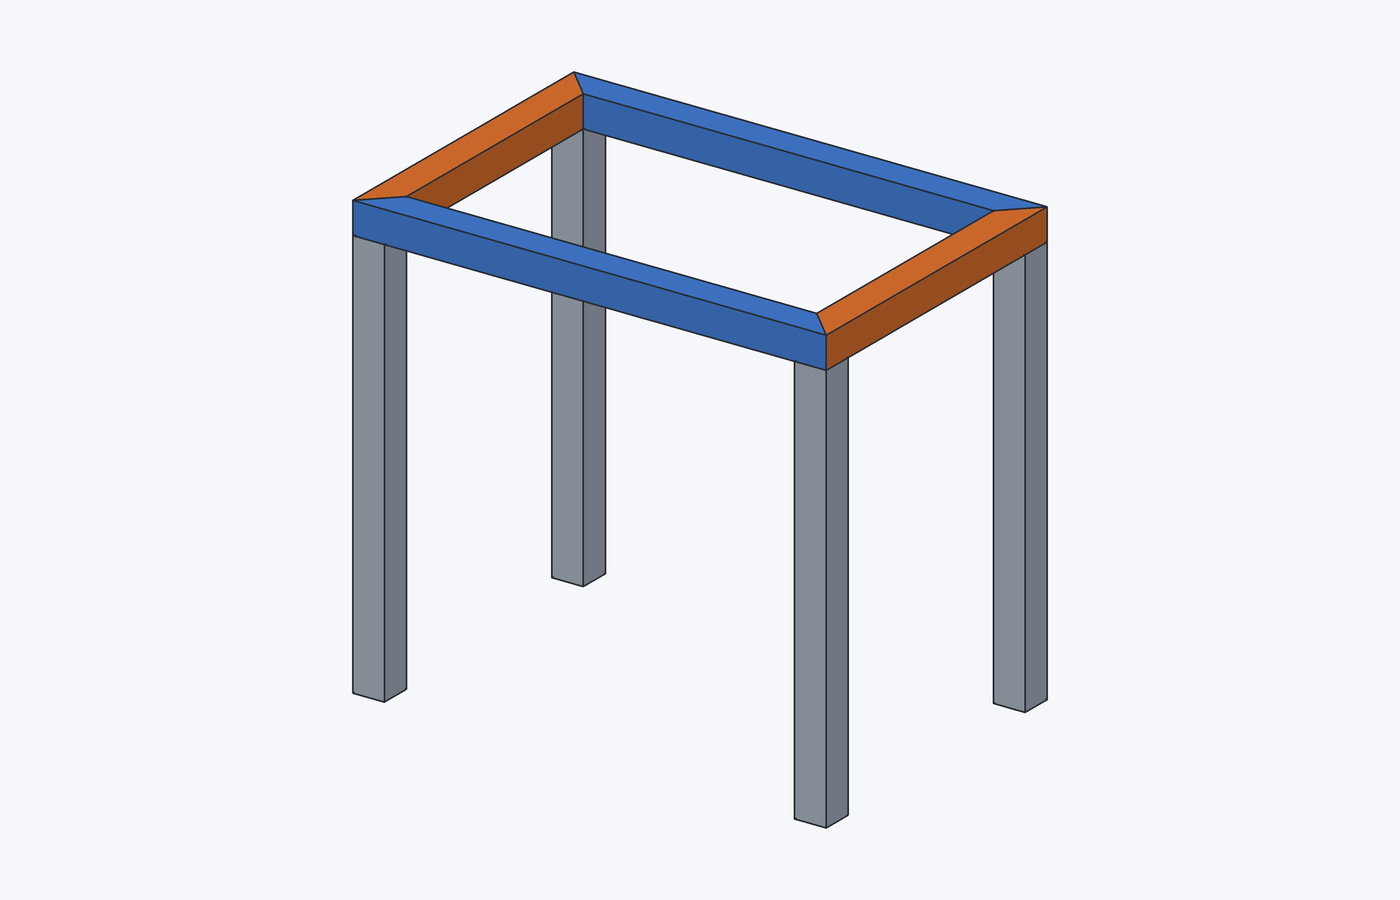
\includegraphics[width=\linewidth]{fig/frame_weldment.png}
\end{minipage}\hfill
\begin{minipage}{0.48\linewidth}
\small
\begin{tabular}{@{}lccc@{}}
\toprule
Member & Qty & Length (outer/inner) & Ends\\
\midrule
Top, long & 2 & 300 / 260 & 45/45\\
Top, short & 2 & 200 / 160 & 45/45\\
Leg & 4 & 260 & 0/0\\
\bottomrule
\end{tabular}\\[4pt]
{\footnotesize 20$\times$20 profile. Generated by \file{render\_roadmap.py}; the fused frame is a valid solid.}
\end{minipage}
\caption{Mitred top frame on butt-jointed legs, and its cut list.}
\label{fig:frame}
\end{figure}

\paragraph{Theory: mitre plane.} Two members meet at corner $\mathbf c$ with unit directions
$\hat{\mathbf d}_1$ (incoming) and $\hat{\mathbf d}_2$ (outgoing). The mitre plane passes through $\mathbf c$
with normal
\[
  \mathbf n=\frac{\hat{\mathbf d}_1+\hat{\mathbf d}_2}{\lVert\hat{\mathbf d}_1+\hat{\mathbf d}_2\rVert},
\]
which bisects the turn. Each member is cut by the half-space on its own side. With turn angle
$\alpha=\arccos(\hat{\mathbf d}_1\!\cdot\hat{\mathbf d}_2)$, the cut is $\alpha/2$ from square, so a
90$^\circ$ corner gives 45$^\circ$. For profile width $w$, the outer edge is longer than the centre line by
$\tfrac{w}{2}\tan\tfrac{\alpha}{2}$ at each mitred end, and the inner edge shorter by the same amount. With
$w=20$ the centre lines are 280 and 180\,mm, which gives the 300/260 and 200/160 pairs above.

%----------------------------------------------------------------------
\subsection{BW-MOD-08 --- Surfacing parity}
%----------------------------------------------------------------------

\begin{epic}{MOD-08}{Surfacing parity}{M5}{\stTodo}{(new)}
Fill the gaps next to the Surface workbench: trim and untrim by curve or surface, patch (n-sided, with
continuity per edge), extend, stitch into a solid, replace face, and thicken. Add \textbf{continuity
analysis} (zebra stripes, curvature comb, deviation map), which is how surfacing is checked in Fusion and
SolidWorks.
\emph{Acceptance:} a surface benchmark set rebuilt to the stated G1/G2 continuity, and thickened into a
valid solid.
\end{epic}

\paragraph{Theory: continuity.} Two surfaces meeting along a curve are $G^0$ if positions match, $G^1$ if
tangent planes match ($\mathbf n_1=\pm\mathbf n_2$ along the curve), and $G^2$ if normal curvatures match in
every direction. Zebra stripes are reflection lines of a striped environment. A stripe stays continuous
across a $G^1$ joint, and stays continuous \emph{and} smooth across $G^2$. That makes them a fast visual test
of the next-higher order. The tolerances checked are angular ($\le0.1^\circ$ for $G^1$) and relative curvature
($\le5\%$ for $G^2$).

%----------------------------------------------------------------------
\subsection{BW-MOD-09 --- Freeform (subdivision / T-spline-like)}
%----------------------------------------------------------------------

\begin{epic}{MOD-09}{Freeform}{M5}{\stTodo}{(new)}
A \textbf{Form body} like Fusion's Form workspace: start from a primitive cage, push and pull faces, edges and
vertices, extrude, crease, and mirror. The result converts to a B-spline B-rep solid that the rest of FreeCAD
can use. T-splines are proprietary, so the open path is \textbf{Catmull--Clark subdivision}, for example via
OpenSubdiv (Apache-2.0) \verify, with conversion to bicubic patches.
\emph{Acceptance:} a drone canopy modelled as a cage and exported as a valid STEP solid.
\end{epic}

\paragraph{Theory.} One Catmull--Clark step creates a face point $\mathbf f$ (the face centroid) and an edge
point $\mathbf e=\tfrac14(\mathbf v_1+\mathbf v_2+\mathbf f_1+\mathbf f_2)$, and moves each vertex of
valence $n$ to
\[
  \mathbf v'=\frac{\mathbf F+2\mathbf R+(n-3)\mathbf v}{n},
\]
with $\mathbf F$ the mean of adjacent face points and $\mathbf R$ the mean of adjacent edge midpoints. On
regular regions (quads, valence 4) the limit surface \emph{is} a uniform bicubic B-spline. Those patches
convert exactly to \code{Geom\_BSplineSurface}. Around extraordinary vertices ($n\neq4$) the limit surface
is not a finite B-spline, so conversion uses $G^1$ approximating patches (Gregory-type) within a tolerance,
and that tolerance is reported. Creases set sharp rules on tagged edges.

%----------------------------------------------------------------------
\subsection{BW-MOD-10 --- Mesh to solid}
%----------------------------------------------------------------------

\begin{epic}{MOD-10}{Mesh to solid}{M5}{\stTodo}{(new)}
A pipeline from STL, 3MF or scan to an editable solid: \textbf{repair} (holes, non-manifold edges, flipped
normals), \textbf{segment} into regions, \textbf{fit} planes, cylinders, cones and spheres, then
\textbf{rebuild} as intersecting analytic faces, or as features where they are recognised. A faceted solid
(\code{Part\_ShapeFromMesh}, which exists) remains the fallback.
\emph{Acceptance:} a scanned bracket becomes a solid with analytic faces within 0.1\,mm of the scan.
\end{epic}

\paragraph{Theory: RANSAC fitting.} To fit a primitive needing $s$ points (3 for a plane) to a region
where a fraction $w$ of points are inliers, the probability that $k$ random samples all fail is
$(1-w^s)^k$. Success with probability $p$ therefore needs $k=\lceil\log(1-p)/\log(1-w^s)\rceil$ samples.
For a plane with $w=0.5$ and $p=0.99$, that is $k=35$. Regions are grown from the best model, removed, and
the search repeats. Deviation is reported as the RMS and maximum point-to-surface distance.

%----------------------------------------------------------------------
\subsection{BW-MOD-11 --- Inspect tools}
%----------------------------------------------------------------------

\begin{epic}{MOD-11}{Inspect tools}{M1}{\stTodo}{FCB-P2R-07, (new)}
Measure (exists), \textbf{mass, centre of gravity and inertia} (extends \code{MeasureCOM}), \textbf{section
analysis} that stays in the model, \textbf{curvature/zebra} (shared with \eref{MOD-08}), \textbf{draft
analysis}, a \textbf{3D-print overhang map} against a build direction, and a \textbf{wall-thickness} map.
\emph{Acceptance:} mass and CG match a hand-calculated fixture; the overhang map flags the expected faces on a
printed part.
\end{epic}

\paragraph{Theory: overhang.} For build direction $\mathbf b$ (unit, up) and face normal $\mathbf n$, a
downward-facing region needs support when its angle from the horizontal is below the critical angle
$\theta_c$ (typically 45$^\circ$ for FDM), that is when
\[
  \mathbf n\cdot(-\mathbf b) > \cos\theta_c .
\]
The map colours each tessellation facet by $\mathbf n\cdot(-\mathbf b)$. Draft analysis is the same test
against a pull direction with $\theta_c$ equal to the draft angle. \textbf{Mass properties} are integrals
over the solid. For $N$ parts with masses $m_i$, centres $\mathbf c_i$ and inertia tensors $I_i$ about their
own centres, the assembly CG is $\bar{\mathbf c}=\sum m_i\mathbf c_i/\sum m_i$, and the parallel-axis theorem
gives $I=\sum_i\big(I_i+m_i(\lVert\mathbf r_i\rVert^2E-\mathbf r_i\mathbf r_i^{\!\top})\big)$ with
$\mathbf r_i=\mathbf c_i-\bar{\mathbf c}$ (see \eref{ROB-03}).

%----------------------------------------------------------------------
\subsection{BW-MOD-12 --- Sketcher parity audit}
%----------------------------------------------------------------------

\begin{epic}{MOD-12}{Sketcher parity audit}{M1}{\stTodo}{(new)}
Sketcher is mature, but full parity needs a checked list. Compare it against Fusion and SolidWorks sketch tools:
slots, conics, text, offset and project/include, sketch patterns, dimension-driven parameters, constraint
inference while drawing, and sketch-level mirror and fillet behaviours. Close the five most-used gaps.
\emph{Acceptance:} gap list approved; top five gaps closed.
\end{epic}
